\documentclass{article}
\usepackage{amsmath, amsfonts}
\usepackage{graphicx}

\title{COMP2120 Assignment 2}
\author{YUAN Wenxuan (UID: 3036292740)}
\date{\today}

\begin{document}

\maketitle

\subsection*{Problem 1}

This program adds from 1 to 9 together and store the result in memory, \\
thus the result is $\sum_{i=1}^{9} = 45$.

\subsection*{Problem 2}

The final result in P is 0x00000014, whose decimal value is 20. \\
This program adds 5 for 4 times, thus the result is $4 \times 5 = 20$.

\subsection*{Screenshot}
\begin{figure}[htbp]
    \centering
    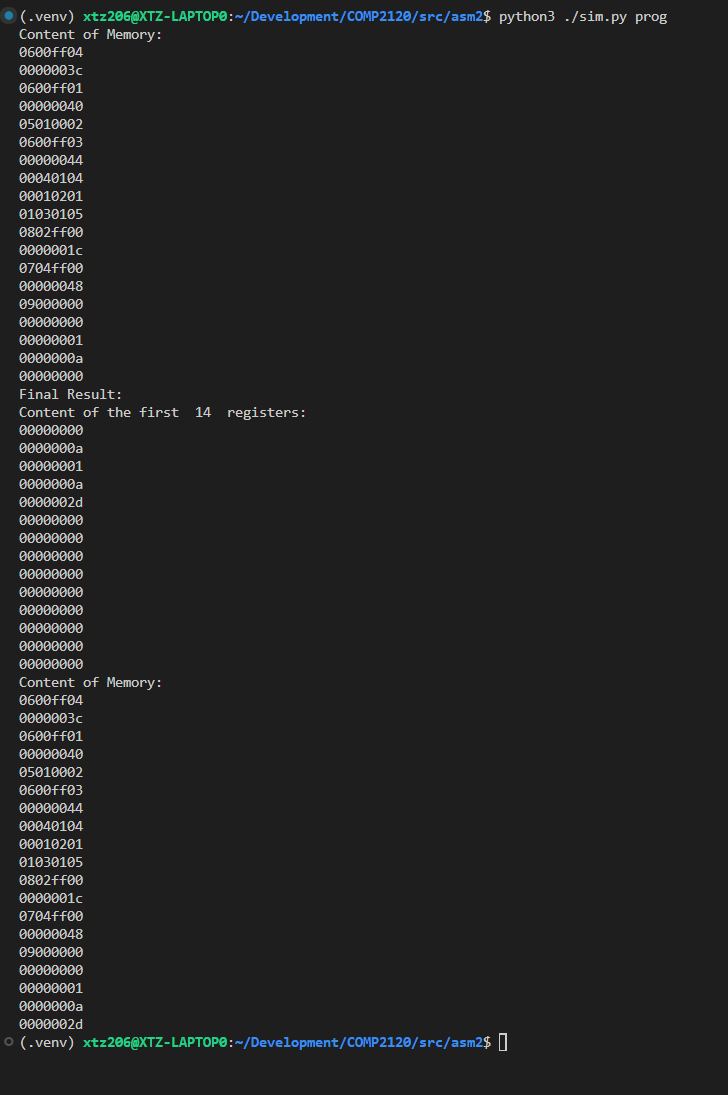
\includegraphics[height=0.7\textwidth]{../../media/asm2/asm2.png}
\end{figure}
% The full program output is too long to be fully captured.


\end{document}
